\documentclass[12pt]{book}
\usepackage{amsmath}
\usepackage{bm}
\usepackage{amsfonts}
\usepackage{setspace}
\usepackage{helvet}
\usepackage{graphicx}
\graphicspath{ {./images/} }
\renewcommand{\familydefault}{\sfdefault}
\doublespacing

\newtheorem{definition}{Definition}[section]

\title{The Singular Value Decomposition}
\author{David Blair}

\begin{document}
	
	\section{Introduction}
	For this project, we will be looking at a matrix factorisation known as the singular value decomposition (SVD). We will start by building up an intuitive understanding of the underlying concepts in linear algebra (see figure ). This will lead into another form of matrix factorisation known as the eigenvalue decomposition which will assist in our proof of the existence of the SVD. 
	
	\section{Types of Matrix}
	There are a few different type of matrices that are applicable to this project. We will provide a formal definition of each matrix and a simpler explanation where it seems necessary. We may occasionally provide code snippets if it is deemed to be useful.   
	
	\subsection{Rectangular Matrix}
	A rectangular matrix is a matrix in which the number of rows is not equal to the number of columns. This is in contrast to a square matrix in which the number of rows and columns are equal.
	
	\subsection{Symmetric Matrix}
	A symmetric matrix $\bm{A}$ is a square matrix where $\bm{A}^{\top} = \bm{A}$ and where $\bm{A}^{\top}$ denotes the transpose where $a_{ij} = a_{ji}$. In other words, the matrix is symmetric about the diagonal line from the top left element to the bottom right element. For example, below is an example of a symmetric matrix:
	
	\begin{align}
		\begin{bmatrix}
			96 & 16 & 38 & 8 & 42 \\
			16 & 60 & 77 & 88 & 99 \\
			38 & 77 & 10 & 11 & 12 \\
			8 & 88 & 11 & 13 & 14 \\
			42 & 99 & 12 & 14 & 15
		\end{bmatrix}
	\end{align}
	
	\subsection{Diagonal Matrix}
	Consider a matrix $\bm{A}$ in which each element is given by $a_{ij}$. A diagonal matrix is a square matrix where $a_{ij} = 0$ when $i \ne j$ and elements where $i = j$ may or may not be zero. Below is the general form of a diagonal matrix:
	
	\begin{align}
		\bm{A} = \begin{bmatrix}
			a_{1,1} & 0 & 0 & \cdots & 0 \\
			0 & a_{2,2} & 0 & \cdots & 0 \\
			0 & 0 & a_{3,3} & \cdots & 0 \\
			\vdots & \vdots & \vdots & \ddots & \vdots \\
			0 & 0 & 0 & \cdots & a_{n,n}
		\end{bmatrix}
		\label{matrix_type:diagonal}
	\end{align}
	
	A diagonal matrix is especially useful for performing common matrix operations. Given an $n \times n$ diagonal matrix represented as $\operatorname{diag}(a_1, a_2, a_3, \ldots, a_n)$, the determinant can be calculated as follows:
	
	\begin{align}
		\sum_{i=1}^n a_i
	\end{align}
	
	In other words, the determinant of a diagonal matrix is the product of its diagonal elements. Given the matrix $\bm{A}$ from equation \ref{matrix_type:diagonal}, its inverse can be calculated as follows: 
	
	\begin{align}
		\bm{A}^{-1} = \begin{bmatrix}
			\frac{1}{a_{1,1}} & 0 & 0 & \cdots & 0 \\
			0 & \frac{1}{a_{2,2}} & 0 & \cdots & 0 \\
			0 & 0 & \frac{1}{a_{3,3}} & \cdots & 0 \\
			\vdots & \vdots & \vdots & \ddots & \vdots \\
			0 & 0 & 0 & \cdots & \frac{1}{a_{n,n}}
		\end{bmatrix}
	\end{align}
	
	And to raise a diagonal matrix to a power $p$, you can simply take each diagonal element to the power of $p$:
	
	\begin{align}
		\bm{A}^p = \begin{bmatrix}
			a_{1,1} & 0 & 0 & \cdots & 0 \\
			0 & a_{2,2} & 0 & \cdots & 0 \\
			0 & 0 & a_{3,3} & \cdots & 0 \\
			\vdots & \vdots & \vdots & \ddots & \vdots \\
			0 & 0 & 0 & \cdots & a_{n,n}
		\end{bmatrix}^p = \begin{bmatrix}
			a_{1,1}^p & 0 & 0 & \cdots & 0 \\
			0 & a_{2,2}^p & 0 & \cdots & 0 \\
			0 & 0 & a_{3,3}^p & \cdots & 0 \\
			\vdots & \vdots & \vdots & \ddots & \vdots \\
			0 & 0 & 0 & \cdots & a_{n,n}^p
		\end{bmatrix}
	\end{align}
	
	These operations are simple to perform, both manually and most importantly, computationally. In many programming languages or packages that allow for linear algebra, if you explicitly define a matrix as being a diagonal matrix and attempt to computer the inverse, determinant or raise it to a power, you can gain great improvements in terms of how quickly the code can execute.
	
	\section{Vector Space}
	A vector space is an algebraic structure that consists of a set of vectors and two operations defined on these vectors: vector addition and scalar multiplication. The elements of the vector space are called vectors, which can be added together and multiplied by numbers, called scalars. The operations of vector addition and scalar multiplication must satisfy a set of axioms, which ensure that the resulting vectors remain within the vector space. 
	
	Lets consider the formal definition of a vector space:
	\begin{definition}[Vector Space]
		\normalfont A real-valued $\textit{vector space}$ $V = (V, +, \cdot)$ is a set $\mathcal{V}$ with two operations:
		\begin{align}
			+: \mathcal{V} &\times \mathcal{V} \rightarrow \mathcal{V} \hspace{10pt} (\text{Inner Operation}) \\
			\cdot: \mathbb{E} &\times \mathcal{V} \rightarrow \mathcal{V} \hspace{10pt} (\text{Outer Operation})
		\end{align}
		where:
		\begin{enumerate}
			\item $(\mathcal{V}, +)$ is an Abelian group
			\item Distributivity: 
			\begin{enumerate}
				\item $\forall \lambda \in \mathbb{R}, \textbf{x}, \textbf{y} \in \mathcal{V}: \lambda \cdot \textbf{x} + \lambda \cdot \textbf{y}$
				\item $\forall \lambda, \psi \in \mathbb{R}, \textbf{x} \in \mathcal{V}: (\lambda + \psi) \cdot \textbf{x} = \lambda \cdot \textbf{x} + \psi \cdot \textbf{x}$
			\end{enumerate} 
			\item Associativity (outer operation): $\forall\lambda, \psi \in \mathbb{R}, \textbf{x} \in \mathcal{V}: \lambda \cdot (\psi \cdot \textbf{x}) = (\lambda\psi)\cdot\textbf{x}$
			\item Neutral element with respect to the outer operation: $\forall \textbf{x} \in \mathcal{V}: 1 \cdot \textbf{x} = \textbf{x}$
		\end{enumerate}
	\end{definition}
	
	It will be helpful to describe a vector space by comparing it to groups. The operation of adding vectors together in a vector space is called the "inner operation," and it behaves like the addition operation in a group. This means that the order in which you add the vectors doesn't matter (e.g. $(u + v) + w = u + (v + w)$). In other words, the inner operation of vector addition is associative, just like the addition operation in a group.
	
	The operation of multiplying a vector by a scalar in a vector space is called the "outer operation." This operation has to follow two rules: it must be "distributive" over the inner operation of vector addition, and it must be "associative." Distributivity means that you can "distribute" the scalar multiplication over the vectors, so instead of adding the vectors together and then multiplying by the scalar, you can first multiply each vector by the scalar and then add the resulting vectors together (e.g. $a \cdot (b + c) = (a \cdot b) + (a \cdot c)$). Associativity means that the order in which you perform the scalar multiplications doesn't matter (e.g. $(a \cdot b) \cdot c = a \cdot (b \cdot c)$).
	
	Finally, the vector space must have a "neutral element," which is a scalar that when multiplied by a vector leaves the vector unchanged. This is similar to the identity element in a group, which is an element that when combined with another element using the group operation leaves the other element unchanged.
	
	Therefore, you can think of a vector space as a group because both involve a set of elements and an operation which together satisfy certain conditions. However, a vector space is a more general structure that includes the additional operation of scalar multiplication, which must satisfy the axioms of distributivity and associativity.
	
	\section{Linear Independence}
	``Linear independence" refers to a property of a set of vectors in a vector space. It can be understood through the process of constructing a "linear combination" of the vectors, which involves performing scalar multiplication and vector addition on the vectors. This concept is often visualized using geometric representations of the vectors.
	
	\begin{definition}[Linear Combination]
		\normalfont	Consider a vector space $\textit{V}$ and a finite number of vectors $\boldsymbol{x}_i,\ldots,\boldsymbol{x}_k \in \textit{V}$. Then, every $\boldsymbol{v} \in \textit{V}$ of the form
		\begin{align}
			\boldsymbol{v} = \lambda_1\boldsymbol{x}_1 + \cdots + \lambda_k\boldsymbol{x}_k =  \sum_{i=1}^{k} \lambda_i\boldsymbol{x}_i \in \textit{V}
		\end{align}
		with $\lambda_1,\ldots,\lambda_k \in \mathbb{R}$ is a $\textit{linear combination}$ of the vectors $\boldsymbol{x}_1,\cdots,\boldsymbol{x}_k$.
	\end{definition}
	
	Linear independence is a specific case of the linear combinations of a set of vectors:
	
	\begin{definition}[Linear (In)dependence]
		\normalfont Let us consider a vector space $\textit{V}$ with $k \in \mathbb{N}$ and  $\boldsymbol{x}_1,\cdots,\boldsymbol{x}_k \in \mathit{V}$. If there is a non-trivial combination, such that $\textbf{0} = \sum_{i=1}^{k} \lambda_i\boldsymbol{x}_i$ with at least one $\lambda_i \ne 0$, the vectors  $\boldsymbol{x}_1,\cdots,\boldsymbol{x}_k$ are $\textit{linearly dependent}$. 
	\end{definition}
	
	When examining a set of vectors in a vector space, we consider the possible linear combinations that can be constructed from the set. For example, consider the set of column vectors $(1, 0)$ and $(0, 1)$ in $\mathbb{R}^2$. We can generate any vector in $\mathbb{R}^2$ using linear combinations of these vectors (see figure \ref{fig:linear_combinations}), and it is not possible to find a non-trivial linear combination that results in the zero vector. In other words, the set of vectors is linearly independent. We will explore this concept and related ideas in the following sections.
	
	\begin{figure}[h]
		\centering
		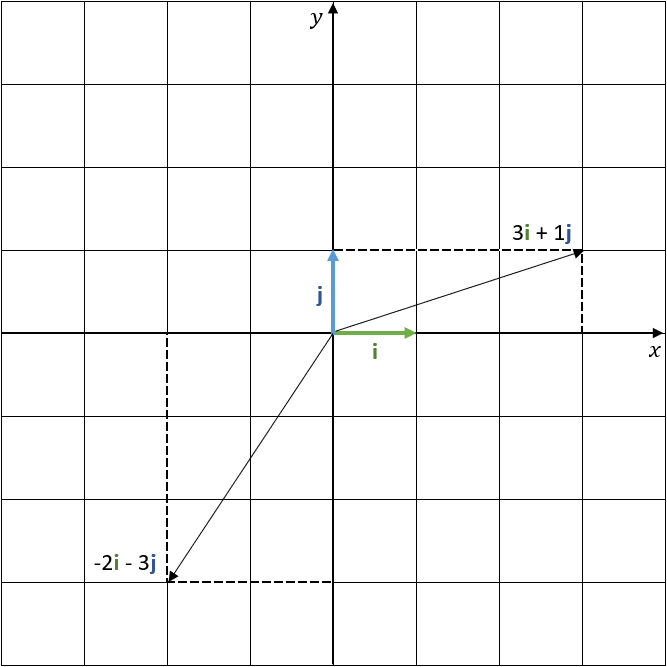
\includegraphics[scale=0.37]{linear_combinations.png}
		\caption{Linear Combinations in $\mathbb{R}^2$.}
		\label{fig:linear_combinations}
	\end{figure}
	
	\subsection{Basis and Rank}
	
	Having introduced the concepts of linear combinations and linear independence, we can now delve into the specific language and ideas associated with these concepts.
	
	\subsubsection{Generating Set and Basis}
	\begin{definition}[Generating Set and Span]
		\normalfont Consider a vector space $\textit{V} = (\mathcal{V}, +, \cdot)$ and set of vectors $\mathcal{A} = \{\boldsymbol{x}_1,\ldots,\boldsymbol{x}_k\} \subseteq \textit{V}$. If every vector $\boldsymbol{v} \in \mathit{V}$ can be expressed as a linear combination of vectors of $\boldsymbol{x}_1,\ldots,\boldsymbol{x}_k$, $\mathcal{A}$ is called the generating set of $\textit{V}$. The set of all linear combinations of vectors in $\mathcal{A}$ is called the span of $\mathcal{A}$. If $\mathcal{A}$ spans the vector space $\textit{V}$, we write $\textit{V} = span[\mathcal{A}]$. 
	\end{definition}

	\begin{figure}[h]
		\centering
		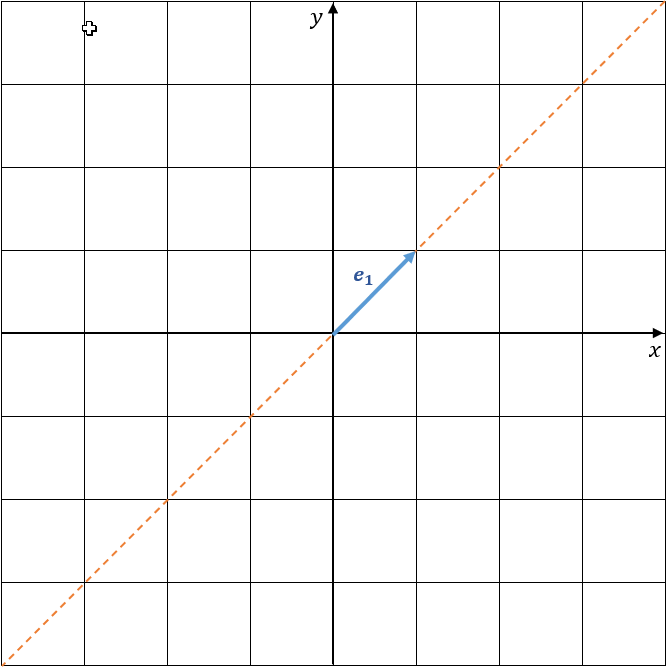
\includegraphics[scale = 0.37]{span.png}
		\caption{A base vector $\textbf{e}_1$ with its span (orange line).}
		\label{fig:span}
	\end{figure}
	
	The above definitions have some interesting visual interpretations in the context of vector spaces and sets of vectors. In figure \ref{fig:span}, all points along the orange line can be represented as a linear combination of $e_1$ Consider a vector space $\textit{V} = (\mathcal{V}, +, \cdot)$ containing a set of vectors $\mathcal{A} = \{\boldsymbol{a}_1,\ldots,\boldsymbol{a}_k\}$. If it is possible to generate every vector in $\mathcal{A}$ using linear combinations of a given set of vectors $\mathcal{B} = \{\boldsymbol{b}_1,\ldots,\boldsymbol{b}_m\}$, then we can say that $\mathcal{B}$ is the generating set of $\textit{V}$. In other words, the set of vectors $\mathcal{B}$ is sufficient to "generate" all of the vectors in $\mathcal{A}$ through the process of linear combination. In our example, we can say that the vector space would contain all vectors along the orange line.
	
	On the other hand, if we start with a set of vectors $\mathcal{C} = \{\boldsymbol{c}_1,\ldots,\boldsymbol{c}_n\}$ and consider all of the possible linear combinations that can be constructed from this set, the vector space of these linear combinations is called the span of $\mathcal{C}$. The span of a set of vectors represents the full range of vectors that can be generated by taking linear combinations of the set.
	
	We can see that a generating set and the span of a set of vectors are two sides of the same concept. A generating set specifies the set of vectors that can be used to generate all vectors in a vector space, while the span of a set of vectors represents the full range of vectors that can be generated from the set through linear combination.

	\begin{figure}[h]
		\centering
		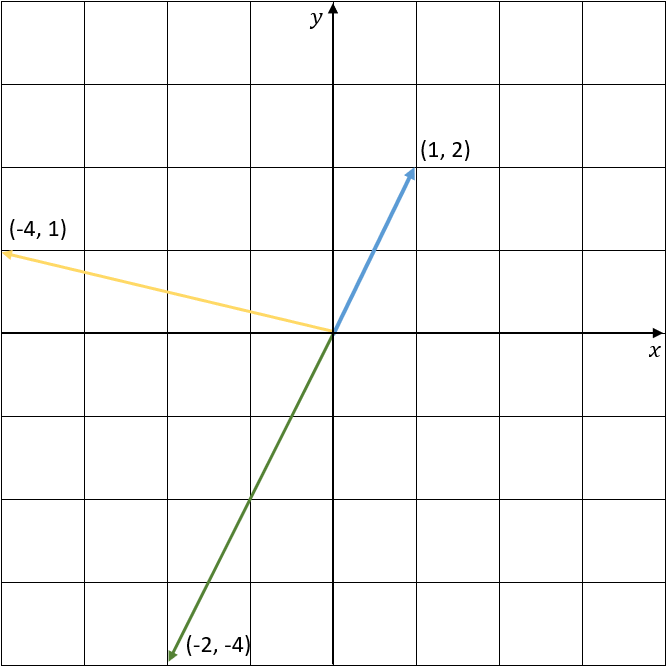
\includegraphics[scale = 0.37]{linear_dependence.png}
		\caption{A plot of a set of linearly dependent vectors.}
		\label{fig:linear_dependent}
	\end{figure}
	
	We can now bring together the various concepts introduced earlier to understand the relationship between linear independence and the span of a set of vectors. Recall that a set of vectors is linearly independent if no non-trivial linear combination of the vectors results in the zero vector. When we consider the span of a set of linearly dependent vectors, we observe an interesting property: it is possible to remove one or more vectors from the set without affecting the span of the set. Consider the following set of vectors $\mathcal{A}$:
	
	\begin{align}
		\mathcal{A} = \left\{\begin{pmatrix} 1 \\ 2 \end{pmatrix},\begin{pmatrix} -2 \\ -4 \end{pmatrix},\begin{pmatrix} -4 \\ -1 \end{pmatrix} \right\}
	\end{align}
	
	 In figure \ref{fig:linear_dependent} the plot of each vector is given. You can see that the span of this set of vectors is $\mathbb{R}^2$ in that every vector in $\mathbb{R}^2$ can be represented as a linear combination of vectors from the set $\mathcal{A}$. If we are able to remove a vector from this set such that the span remains unchanged, the set of vectors are linearly dependent. In this case, we can see that since $(1, 2)^{\top}$ and $(-2, -4)^{\top}$ sit on the same line, we are able to remove either one and the full set of linear combinations will continue to span $\mathbb{R}^2$. We can also consider this algebraically: 
	 
	 \begin{align}
	 	\mathbf{v} &= \alpha \begin{pmatrix} 1 \\ 2 \end{pmatrix} + \beta \begin{pmatrix} -2 \\ -4 \end{pmatrix} + \omega \begin{pmatrix} -4 \\ -1 \end{pmatrix} \\
	 	&= \alpha \begin{pmatrix} 1 \\ 2 \end{pmatrix} - 2\beta \begin{pmatrix} 1 \\ 2 \end{pmatrix} + \omega \begin{pmatrix} -4 \\ -1 \end{pmatrix} \\
	 	&= (\alpha - 2\beta) \begin{pmatrix} 1 \\ 2 \end{pmatrix} + \omega \begin{pmatrix} -4 \\ -1 \end{pmatrix} \\
	 \end{align}
 
 	What is shown above is that if I have a vector $\mathbf{v}$ that is a linear combination of vectors in the set $\mathcal{A}$, I can actually express the same vector as a combination of just vectors $(1, 2)^{\top}$ and $(-4, -1)^{\top}$. This also follows on from our formal definition of linear independence since vectors which behave in this way form linear combinations that may produce the zero vector. Therefore, the following set of vectors is said to be linearly independent:
 	
 	\begin{align}
 		\mathcal{A}_1 = \left\{\begin{pmatrix} 1 \\ 2 \end{pmatrix},\begin{pmatrix} -4 \\ -1 \end{pmatrix} \right\}
 	\end{align}
	
	\begin{definition}[Basis]
		\normalfont Consider a vector space $\textit{V} = (\textit{V}, +, \cdot)$ and $\mathcal{A} \subseteq \mathcal{V}$. A generating set $\mathcal{A}$ of $\textit{V}$ is called $\textit{minimal}$ if there exists no smaller set $\tilde{A} \subseteq \mathcal{A} \subseteq \mathcal{V}$ that spans $\textit{V}$. Every linearly independent generating set of $\textit{V}$  is minimal and is called a $\mathit{basis}$ or $\textit{V}$.
	\end{definition}
	
	A particularly useful type of linearly independent vector set is one that can serve as a generating set for a vector space. In other words, the set of vectors is sufficient to generate all vectors in the vector space through linear combination. If such a set is also minimal in the sense that no vectors can be removed without reducing the span, it is called a basis for the vector space. An example of a vector space that is familiar to many people is $\mathbb{R}^2$. In this vector space, the basis consists of the column vectors $(1, 0)$ and $(0, 1)$. These vectors can be combined linearly to generate all vectors in $\mathbb{R}^2$, and no vectors can be removed from the set without reducing the span of the vector space.
	
	In our example from above, we would say that $\mathcal{A}_1$ forms a basis for $\mathbb{R}^2$ since it is a generating set of the vector space where no vectors can be removed without reducing the span. 
	
	The concept of a basis is important because it allows us to represent any vector in the vector space using a unique combination of the basis vectors. This property, known as the basis representation of a vector, is useful for many applications, such as solving systems of linear equations and performing linear transformations.
	
	\begin{definition}[Rank]
		\normalfont The number of linearly independent columns of a matrix $\textbf{A} \in \mathbb{R}^{m \times n}$ equals the number of linearly independent rows and is called the $\textit{rank}$ of $\textbf{A}$ and is denoted by $rk(\textbf{A})$.
	\end{definition}
	
	The rank can be viewed by considering a system of linear equations and examining the relationships between the equations. If one equation can be derived from a combination of other equations in the system through the use of multiplication and/or addition, that equation is considered redundant because it does not provide any new information or insights that would help to solve the system.
	
	This concept also applies when representing the system as a matrix to utilise Gaussian elimination as a method of solution. In this case, the rank of the matrix is determined by the number of linearly independent rows or columns, which if viewed as a set of vectors, cannot be expressed as linear combinations of other vectors within the set. The rank of a matrix is an important property that reflects the number of dimensions required to fully represent the information contained within the matrix. If you consider the rows or columns of a matrix to be a set of vectors, the subset of vectors required to form a linearly independent set is also the number of linearly independent rows and columns of the matrix and this is what we would describe as the rank of a matrix.
	
	\begin{definition}[Row Space]
		\normalfont Let $\mathcal{C}$ be a set of vectors of length $m$ where each vector is a row of a matrix $\textbf{A} \in \mathbb{R}^{m \times n}$. The row space of the matrix $\textbf{A}$ is the vector space of the $span$ of the set of vectors $\mathcal{C}$. 
	\end{definition}
	
	\begin{definition}[Column Space]
		\normalfont Let $\mathcal{C}$ be a set of vectors of length $n$ where each vector is a column of a matrix $\textbf{A} \in \mathbb{R}^{m \times n}$. The column space of the matrix $\textbf{A}$ is the vector space of the $span$ of the set of vectors $\mathcal{C}$. 
	\end{definition}
	
	It has been established through our discussion that the row space and column space of a matrix are connected in a meaningful way. It is known that the concept of linear independence is related to the span of a matrix. Specifically, when a set of vectors is linearly dependent, it is possible to remove a vector from the set without reducing the span. In contrast, removing a vector from a linearly independent set of vectors will affect the span. In addition, we have found that the rank of a matrix is determined by the ability to express row or column vectors of the matrix as linear combinations of other row or column vectors in the matrix. As a result, the dimension of the row space is equal to the rank of the matrix. As the number of linearly independent rows is equal to the number of linearly independent columns, the row space and column space have the same dimensions.
	
	\section{Linear Transformation}
	The material covered so far may seem disconnected at times. However, for myself, the topic of linear transformations was when everything began to fall into place. All of the concepts previously discussed are effectively integrated through the study of linear transformations. I give credit to the YouTube channel 3Blue1Brown for providing an intuitive explanation of linear transformations using what we have discussed so far.
	
	Transformations are in essence just functions. In the context of linear algebra, they take in some vector as input and return another vector as the output. By using the word "transformation", it is an indication of the movement from one state to another. 
	
	Lets consider a vector space many of us are familiar with which is $\mathbb{R}^2$. Imagine if we could apply a transformation to every coordinate in this space. Visually, we would see each coordinate move to another coordinate. For our purposes, we will only be concerning ourselves with one particular type of transformation known as linear transformations. Linear transformations are unique in that they follow two conditions:
	
	\begin{enumerate}
		\item when transforming a straight line, the line will remain straight after the transformation.
		\item The zero vector will remain as the zero vector after the transformation. 
	\end{enumerate}
	
\end{document}
